\section{AOP Solutions}
\label{sec:AOPSolutions}

As the concept of AOP has been embraced as a useful extension to classic programming, different AOP solutions have been developed.
Each solution has one or more implementations to demonstrate how the solution is to be used. 
As described by~\cite{elrad:cacm01} these differ primarily in:
\begin{description}[style=nextline,noitemsep]
  \item[How aspects are specified] Each technique uses its own aspect language to describe the concerns;
  \item[Composition mechanism] Each technique provides its own composition mechanisms;
  \item[Implementation mechanism] Whether components are determined statically at compile time or dynamically at run time, the support for verification of compositions, and the type of weaving.
  \item[Use of decoupling] Should the writer of the main code be aware that aspects are applied to his code;
  \item[Supported software processes] The overall process, techniques for reusability, analyzing aspect performance of aspects, is it possible to monitor performance, and is it possible to debug the aspects.
\end{description}

This section will give a short introduction to AspectJ~\cite{kiczales:ecoop01} and Hyperspaces~\cite{ossher:sact01}, which together with Composition Filters~\cite{bergmans:cacm01} are three main AOP approaches.

\subsection{AspectJ Approach}
\label{sec:TheAspectJApproach}

\emph{AspectJ}~\cite{kiczales:ecoop01} is an aspect-oriented extension to the Java programming language.
It is probably the most popular approach to AOP at the moment, and it is finding its way into the industrial software development.
AspectJ has been developed by Gregor Kiczales at Xerox's PARC (Palo Alto Research Center).
To encourage the growth of the AspectJ technology and community, PARC transferred AspectJ to an open Eclipse project.
The popularity of AspectJ comes partly from the various extensions based on it, build by several research groups.
There are various projects that are porting AspectJ to other languages, resulting in tools such as AspectR and AspectC.

One of the main goals in the design of AspectJ is to make it a compatible extension to Java.
AspectJ tries to be compatible in four ways:
\begin{description}[style=nextline,noitemsep]
  \item[Upward compatibility] All legal Java programs must be legal AspectJ programs;
  \item[Platform compatibility] All legal AspectJ programs must run on standard Java virtual machines;
  \item[Tool compatibility] It must be possible to extend existing tools to support AspectJ in a natural way; this includes IDEs, documentation tools and design tools;
  \item[Programmer compatibility] Programming with AspectJ must feel like a natural extension of programming with Java.
\end{description}

AspectJ extends Java with support for two kinds of crosscutting functionality.
The first allows defining additional behavior to run at certain well-defined points in the execution of the program and is called the \emph{dynamic crosscutting mechanism}.
The other is called the \emph{static crosscutting mechanism} and allows modifying the static structure of classes (methods and relationships between classes).
The units of crosscutting implementation are called aspects.
An example of an aspect specified in AspectJ is shown in \autoref{lst:dynamiccrosscuttingexample}.

\begin{lstlisting}[language={[AspectJ]Java},style=floatlisting,%
                   caption={Example of dynamic crosscutting in AspectJ},%
                   label={lst:dynamiccrosscuttingexample}]
aspect DynamicCrosscuttingExample {
  Log log = new Log();

  pointcut traceMethods():
    execution(edu.utwente.trese.*.*(..));

  before() : traceMethods {
    log.write("Entering " + thisJointPoint.getSignature());
  }

  after() : traceMethods {
    log.write("Exiting " + thisJointPoint.getSignature());
  }
}
\end{lstlisting}

The points in the execution of a program where the crosscutting behavior is inserted are called \emph{join points}.
A \emph{pointcut} has a set of join points.
In \autoref{lst:dynamiccrosscuttingexample} is \lstinline|traceMethods| an example of a pointcut definition.
The pointcut includes all executions of any method that is in a class contained by package \lstinline|edu.utwente.trese|.

The code that should execute at a given join point is declared in an advice.
Advice is a method-like code body associated with a certain pointcut.
AspectJ supports \emph{before}, \emph{after} and \emph{around} advice, which specifies where the additional code is to be inserted.
In the example both before and after advice are declared to run at the join points specified by the \lstinline|traceMethods| pointcut.

Aspects can contain anything permitted in class declarations including definitions of pointcuts, advice and static crosscutting.
For example, static crosscutting allows a programmer to add fields and methods to certain classes as shown in \autoref{lst:staticcrosscuttingexample}.

\begin{lstlisting}[language={[AspectJ]Java},style=floatlisting,%
                   caption={Example of static crosscutting in AspectJ},%
                   label={lst:staticcrosscuttingexample},floatplacement=htbp]
aspect StaticCrosscuttingExample {
  private int Log.trace(String traceMsg) {
    Log.write(" --- MARK --- " + traceMsg);
  }
}
\end{lstlisting}

The shown construct is called inter-type member declaration and adds a method \lstinline|trace| to class \lstinline|Log|.
Other forms of inter-type declarations allow developers to declare the parents of classes (super classes and realized interfaces), declare where exceptions need to be thrown, and allow a developer to define the precedence among aspects.

With its variety of possibilities, AspectJ can be considered a useful approach for realizing software requirements.

\subsection{Hyperspaces Approach}

The \emph{Hyperspaces} approach is developed by H.~Ossher and P.~Tarr at the IBM T.J.~Watson Research Center.
The Hyperspaces approach adopts the principle of multi-dimensional separation of concerns~\cite{ossher:sact01}, which involves:
\begin{itemize}[noitemsep]
  \item Multiple, arbitrary dimensions of concerns;
  \item Simultaneous separation along these dimensions;
  \item Ability to dynamically handle new concerns and new dimensions of concern as they arise throughout the software life cycle;
  \item Overlapping and interacting concerns. It is appealing to think of many concerns as independent or orthogonal, but they rarely are in practice.
\end{itemize}

We explain the Hyperspaces approach by an example written in the \emph{Hyper/J} language.
Hyper/J is an implementation of the Hyperspaces approach for Java.
It provides the ability to identify concerns, specify modules in terms of those concerns, and synthesize systems and components by integrating those modules.
Hyper/J uses byte code weaving on binary Java class files and generates new class files to be used for execution.
Although the Hyper/J project seems abandoned and there has not been any update in the code or documentation for a while, we still mention it because the Hyperspaces approach offers a unique AOP solution.

As a first step, developers create hyperspaces by specifying a set of Java class files that contain the code units that populate the hyperspace.
To do this, you create a hyperspace specification, as demonstrated in \autoref{lst:hyperspaces1}.

\begin{lstlisting}[language={[HyperJ]Java},style=floatlisting,%
                   caption={Creation of a hyperspace},label={lst:hyperspaces1},%
                   floatplacement=htbp]
Hyperspace Pacman
  class edu.utwente.trese.pacman.*;
\end{lstlisting}

Hyper/J will automatically create a hyperspace with one dimension---the class file dimension.
A dimension of concern is a set of concerns that are disjoint.
The initial hyperspace will contain all units within the specified package.
To create a new dimension you can specify concern mappings, which describe how existing units in the hyperspace relate to concerns in that dimension, as demonstrated in \autoref{lst:hyperspaces2}.

\begin{lstlisting}[language={[HyperJ]Java},style=floatlisting,%
                   caption={Specification of concern mappings},label={lst:hyperspaces2},%
                   floatplacement=htbp]
package edu.utwente.trese.pacman: Feature.Kernel
operation trace: Feature.Logging
operation debug: Feature.Debugging
\end{lstlisting}

The first line indicates that, by default, all of the units contained within the package \lstinline|edu.utwente.trese.pacman| address the kernel concern of the feature dimension.
The other mappings specify that any method named \lstinline|trace| or \lstinline|debug| address the logging and debugging concern respectively.
These later mappings override the first one.

Hypermodules are based on concerns and consist of two parts.
The first part specifies a set of hyperslices in terms of the concerns identified in the concern matrix.
The second part specifies the integration relationships between the hyperslices.
A hyperspace can contain several hypermodules realizing different modularizations of the same units.
Systems can be composed in many ways from these hypermodules.

\begin{lstlisting}[language={[HyperJ]Java},style=floatlisting,%
                   caption={Defining a hypermodule},label={lst:hyperspaces3},%
                   floatplacement=htbp]
hypermodule Pacman_Without_Debugging
  hyperslices: Feature.Kernel, Feature.Logging;
  relationships: mergeByName;
end hypermodule;
\end{lstlisting}

\autoref{lst:hyperspaces3} shows a hypermodule with two concerns, kernel and logging.
They are related by a \lstinline|mergeByName| integration relationship.
This means that units in the different concerns correspond if they have the same name (\lstinline|ByName|) and that these corresponding units are to be combined (\lstinline|merge|).
For example, all members of the corresponding classes are brought together into the composed class.
The hypermodule results in a hyperslice that contains all the classes without the debugging feature; thus no \lstinline|debug| methods will be present.

The most important feature of the hyperspaces approach is the support for on-demand remodularisation: the ability to extract hyperslices to encapsulate concerns that were not separated in the original code.
Which makes hyperspaces especially useful for evolution of existing software.

\subsection{Composition Filters}
\label{sec:Composition_Filters}

\nomenclature{CF}{Composition Filters}%
\emph{Composition Filters} is developed by M.~Ak\c{s}it and L.~Bergmans at the TRESE group, which is a part of the Department of Computer Science of the University of Twente, The Netherlands.
The composition filters (CF) model predates aspect-oriented programming.
It started out as an extension to the object-oriented model and evolved into an aspect-oriented model.
The current implementation of CF is \Compose*, which covers \dotNET, Java, and C.

One of the key elements of CF is the \emph{message}, a message is the interaction between objects, for instance a method call.
In object-oriented programming the message is considered an abstract concept. In the implementations of CF it is therefore necessary to reify the message.
This \emph{reified message} contains properties, like where it is send to and where it came from.

The concept of CF is that messages that enter and exit an object can be intercepted and manipulated, modifying the original flow of the message.
To do so, a layer called the \emph{interface part} is introduced in the CF model, this layer can have several properties.
The interface part can be placed on an object, which behavior needs to be altered, and this object is referred to as \emph{inner}.

%\begin{figure}
%  \centering
%  \includegraphics[style=thirdheight]{cfmodel}
%  \caption{Components of the composition filters model}
%  \label{fig:cfmodel}
%\end{figure}

There are three key elements in CF: messages, filters, and superimposition.
Messages are sent from one object to another, if there is an interface part placed on the receiver, then the message that is sent goes through the input filters.
In the filters the message can be manipulated before it reaches the inner part, the message can even be sent to another object.
How the message will be handled depends on the filter type.
An output filter is similar to an input filter, the only difference is that it manipulates messages that originate from the inner part.
The latest addition to CF is superimposition, which is used to specify which interfaces needs to be superimposed on which
inner objects.

%\begin{lstlisting}[language=ComposeStar,style=floatlisting,%
%                   caption={Example of a filter module specification},label={lst:concern}]
%concern interfaceSound in pacman {
%  filtermodule beepSound {
%    internals
%      beeper : pacman.ConcernImplementations.Beeper;
%    conditions
%      soundOff : pacman.Game.isSoundOn();
%    inputfilters
%      soundOff_filter : Dispatch = {soundOff => [*.*] *.*};
%      beep_filter : Meta = {
%        [*.eatFood] beeper.eatBeep,
%        [*.eatGhost] beeper.eatGhostBeep,
%        [*.eatVitamin] beeper.powerBeep,
%        [*.pacmanKilled] beeper.bumpGhostBeep }
%  }
%}
%\end{lstlisting}

%The message manipulation mechanism of the CF model is explained by means of an example demonstrated in \autoref{lst:concern}.
%This example uses a dispatch filter and a meta filter.
%When \lstinline|soundOff| is true, the dispatch filter will leave the message as it is, this implies that the message will leave the filter and thus will not come through to the second filter.
%The second filter is a meta filter, if the message is send to the method \lstinline|eatFood|, then the filter status is send as a message to \lstinline|beeper.eatBeep|.
%If the message does not have \lstinline|eatFood| as selector, the filter tries the other options from right to the left until there is a match. If there is no match at all the message will leave the filter unaltered.

%The latest addition to CF is superimposition, which is used to specify crosscuts.
%Crosscuts are made by combining a filter module with a selection of objects, as shown in \autoref{lst:concern1}.
%In the given example the filter module \lstinline|tracingModule| is superimposed on every instance of the classes \lstinline|Pacman|, \lstinline|Ghost|, and \lstinline|World|.

%\begin{lstlisting}[language=ComposeStar,style=floatlisting,%
%                   caption={Example of the use of superimposition},label={lst:concern1}]
%concern Tracing {
%  filtermodule tracingModule { }
%
%  superimposition {
%    selectors
%      withTracing = { C | isClassWithNameInList(C,
%                          ['Pacman', 'Ghost', 'World']) };
%    filtermodules
%      withTracing <- tracingModule;
%  }
%}
%\end{lstlisting}

